%
% main.tex -- Paper zum Thema <thema>
%
% (c) 2018 Nicolas Tobler, Hochschule Rapperswil
%

\chapter{Klima auf anderen Planeten\label{chapter:thema}}
\lhead{Klima auf anderen Planeten}
\begin{refsection}
\chapterauthor{Nicolas Tobler}

\section{Einleitung}
\rhead{Einleitung}
%TODO inlude mercury
\begin{figure}
	% https://www.astrobio.net/news-exclusive/comparing-climates-from-earth-to-exoplanets/
	\centering
	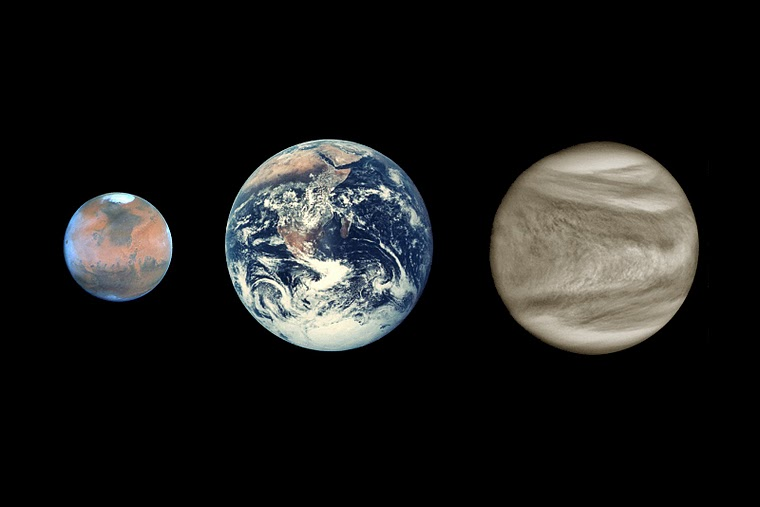
\includegraphics[width=0.7\linewidth, trim={0 3cm 0 3cm},clip]{planeten/Pictures/planets.jpg}
	\caption{Mars, Erde und Venus massstabsgerecht}
\end{figure}



%Verschiedene Organisationen, wie unter anderem Elon Musk's SpaceX, haben sich zum Ziel gemacht, in absehbarer Zukunft den Mars für den Menschen bewohnbar zu machen. Insbesondere sollte der Mars eine erdählnliche Atmosphere erhalte, also terraformed werden. Was auf Computer-generierten bildern ziemlich simpel aussieht, wird sich in realität wahrscheinlich ziemlich schwierig herausstellen. In diesem Kapitel wird die aktuelle lage des Klimas auf dem Mars analysiert und mögliche Wege den Mars zu teraformen auf die Machbarkeit untersucht.

In der Gegenwart

Betrachtet man die vier der Sonne am nächst Stehenden Planeten Merkur, Venus, Erde und Mars, gibt es einige Dinge festzustellen:

%Leben, wasser
Die Erde ist aus heutiger Sicht der einzige Planet der leben aufweist. Das für Leben notwendige flüssige Wasser ist auch nur auf der Erde in grossen Mengen auffindbar. Glücklicherweise lässt das, im Vergleich zu den anderen Planeten, milde Klima einen aktiven Wasserkreislauf zu.
Alle anderen Planeten erfuhren offenbar ein anderes Schicksal.

%Temperatur
Man könnte meinen, dass primär die Distanz der Planeten zur Sonne für das  Klima ausschlaggebend ist. Jedoch nimmt die Temperatur über die Planeten mit der Entfernung zur Sonne nicht stetig ab. Das Klima muss somit auch von anderen Parametern abhängig sein, wie zum Beispiel Durchmesser, Rotation, Vulkanismus, Magnetfeld und viele andere.

Auf Venus, Erde und Mars kann flüssiges Wasser auftreten (Godilooks-Zone).

Ein extremes Klima kann auch dazu führen, dass ein Planet sich irreversibel verändert, indem er zum Beispiel seine Atmosphäre ins All verliert. Wie es vermutlich beim Mars der Fall war.

Könnte es der Erde in Zukunft auch gleichermassen ergehen?

Sind Venus und Mars aufgrund ihrer orbitalen Eigenschaften inhabitabel?

Trotz allen Einwirkungen sind wir in der glücklichen Lage auf der Erde ein mildes Klima vorzufinden. 

Was führt zu wasserlosen Atmosphäre?

%TODO quote syntax?
\vspace{5pt}
\textit{“It may be that conditions for life’s origin aren’t rare, but the hard part is the persistence of habitable conditions.”} \\
\rightline{--- David Grinspoon, Astrobiologe}
\vspace{5pt}
%% https://www.space.com/21234-alien-planets-earth-climate-future.html

\begin{center}
\begin{table}
	\center
	\begin{tabular}{l|c c c c}
                      & Mars    & Erde   & Venus           & Merkur\\
  \hline
  Temperatur (Mittel) & 218 K   & 288 K  & 737 K           & 440 K\\
  Wolken              & $<5\%$ & $68\%$ & $\approx100\%$ & - \\
  Atmosphäre          & $6 \cdot 10^{-3}$ bar & $1$ bar & $92$ bar & $10^{-15}$ bar
	%\hline
	
\end{tabular}
\caption{Planeten im Vergleich}
\end{table}

\end{center}

%Merkur ist in der Tabelle vertreten um zu verdeutlichen, dass nahe an der Sonne nicht direkt eine heisse Mitteltemperatur bedeutet.

\subsection{Ziel}
Dieses Kapitel zeigt ein Modell, wie das Klima eines Planeten mit deren orbitalen Eigenschaften verknüpft werden kann.
Betrachtet wird ein früher Zeitpunkt der Geschichte des Sonnensystems, als die Planeten ähnliche oder annähernd gleiche materielle und Atmosphärische Eigenschaften aufwiesen.
Mit der Annahme, dass grosse Mengen an Wasser auf allen Planeten vorhanden war, besteht auf allen Planeten die gleichen Voraussetzungen für mögliches Leben.
Das gleiche Modell wird mit unterschiedlichen orbitalen Parameter angewendet. Mann kann sich das vorstellen, als nehme man zum Beispiel die Erde, skaliert sie auf Mars-Grösse und setzt sie in den Mars-Orbit. 
Durch eine Simulation des Modells im Zeitbereich sollte dann eine Aussage über den Werdegang der Planeten gemacht werden.

%Dadurch kann der Werdegang der Planeten nachvollzieht werden.

%\subsection{Idee}
%Planeten mit gleichem Modell simulieren
%Orbitale Eigenschaften verwenden


%\subsection{Atmosphereische Eigenschaften}
%
%dünne Atmosphere
%
%Wann und wieso verlor der Mars seine Atmosphäre
%
%Rückgang der Atmosphäre durch Sonnenwind
%	https://www.nasa.gov/press-release/nasa-mission-reveals-speed-of-solar-wind-stripping-martian-atmosphere

\section{Modell}
\rhead{Modell}


	Das Modell muss einige Sachen erfüllen, um eine Aussage machen zu können.

	1. Für alle Planeten geltendes Modell erstellen
	
	2. Modell soll Erdähnliche Bedingungen bewusst erstreben, um zu sehen ob diese auf den Planeten Mars und Venus auch bestehen können.
	
	
	Das hier erarbeitete Modell konzentriert sich nur auf die Strahlungsbillanz und den Wasserkreislauf. Es wird davon ausgegangen, dass das Wasser signifikant für das Klima ist, da atmosphärischer Wasserdampf auf der Erde den grössten Anteil zum Treibhauseffekt beisteuert.
	
Ausserdem befinden sich alle betrachteten Planeten in der Habitablen Zone, auch Bekannt als Goldilocks Zone. Diese beschreibt den Abstandsbereich um die Sonne, in dem flüssiges Wasser dauerhaft auftreten kann.
	Andere klimabestimmenden atmosphärischen Gase wie $\text{CO}_\text{2}$ werden nicht simuliert, um das Modell im gegebenen Rahmen umzusetzen.

%Des Weiteren ist es für den Menschen interessant Planeten mit Erdähnlichen Zuständen anzutreffen.

Zusammengefasst:

 Dazu müssen einige Annahmen getroffen werden:
\begin{itemize}
	\item Gleiche materielle Eigenschaften
	\item Gleiches Vorkommen an Wasser
	\item Wasser hat grösste Auswirkung auf Klima
\end{itemize}			
	
	
Möglichst auf einfachen Physikalischen Gesetzen basieren.	
	
	
Am Schluss müssen freie Parameter abgeschätzt werden, um überhaupt plausible Lösungen zu erreichen.


Abbildung \ref{planeten_model} zeigt eine Übersicht des Modells. Die einzelnen Bestandteile werden im Folgenden beschrieben.

\begin{figure}
	\centering
	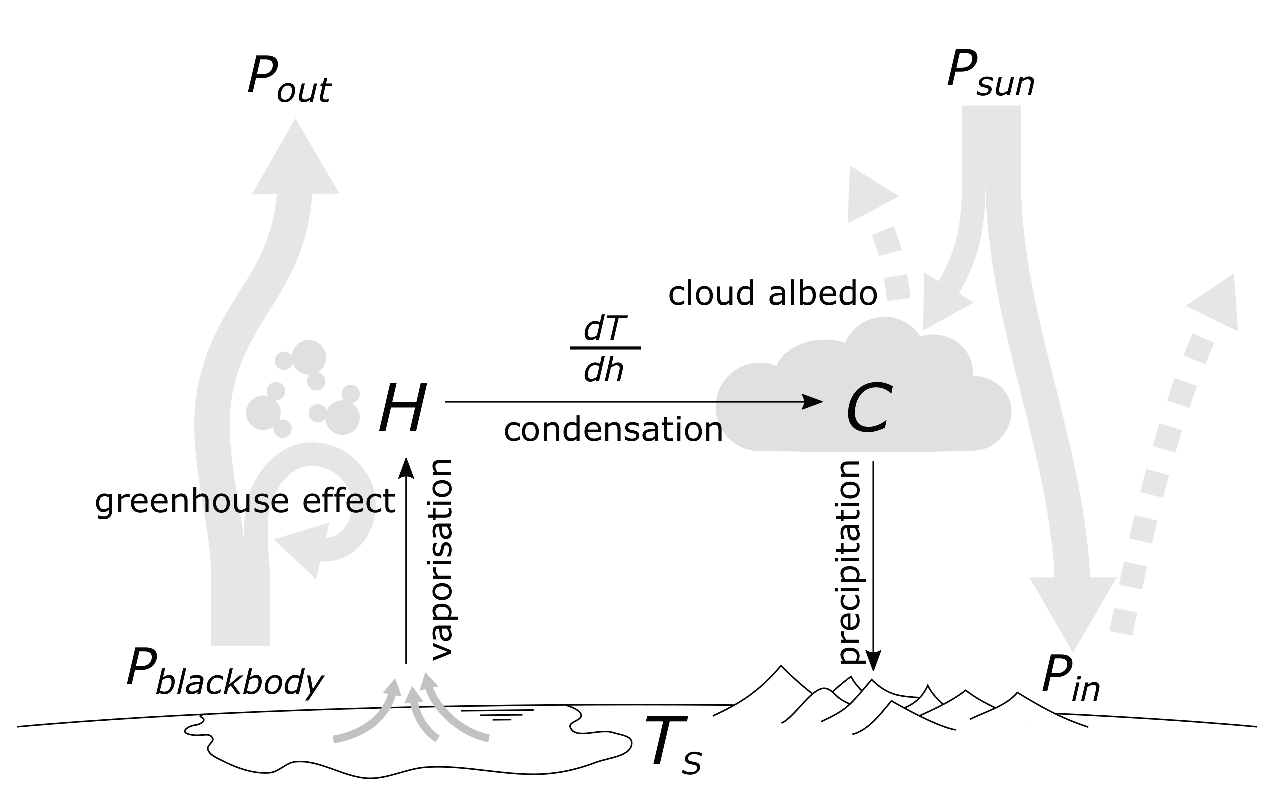
\includegraphics[width=\textwidth]{planeten/Pictures/Model.eps}
	\caption{Modell-Übersicht}
	\label{planeten_model}
\end{figure}

\subsection{Strahlungsbilanz}
%TODO reference
Die Strahlungsbillanz wird in Kapitel \hl{reference needed} ausführlich beschrieben. Das hier verwendeten Modell baut direkt darauf auf.

Damit die Durchschnittstemperatur eines Planeten stabil ist, muss die Leistungsbilanz Null sein. Wie fest sich die Leistungsdifferenz auf die Temperatur auswirkt ist im Modell nicht definiert. Deshalb wird mit dem freien Parameter $\xi_1$ multipliziert. 

\begin{equation}
\dot{T} = \xi_1(P_{\text{in}} - P_{\text{out}})
\end{equation}

%TODO anderer begriff für Aktives Planet-Inneres .. geothermie? (nur für erde)
Die Eintreffende Leistung $P_{in}$ besteht primär aus der absorbierten Sonnenstrahlung. Andere Energiequellen wie ein Aktives Planet-Inneres und die Energie aus Gezeiten wird vernachlässigt. Es gilt:

%TODO P oder S für leistung pro fläche

\begin{equation}
P_{in} = \sigma T_{\astrosun}^4 \left( \frac{R_{\astrosun}}{A_{\text{planet}}} \right) ^2 \cdot (1-\alpha)
\end{equation}

Dabei ist $\sigma$ die Stefan-Boltzmann-Konstante, $T_{\astrosun}$ \& $R_{\astrosun}$ die Oberflächentemperatur und Radius der Sonne, $ A_{\text{planet}}$ die mittlere Distanz des Planeten zur Sonne und $\alpha$ die Albedo des Planeten.

Die Abgestrahlte Leistung besteht praktisch ausschliesslich aus der Black-body Strahlung, welche sich aus der Durchschnittstemperatur $T$ und dem Radius $R$ des Planeten bestimmen lässt. Diese Leistung bleibt jedoch teilweise durch den Treibhauseffekt in der Atmosphäre gefangen. Es gilt: 

\begin{equation}
P_{out} = (4 \pi R^2 \sigma T^4) \epsilon
\end{equation}

Dabei ist $\epsilon$ der Anteil der durchdringenden Leistung.

\subsection{Albedo}

Die Albedo wird als Funktion der prozentualen Wolkenabdeckung $C$ modelliert. Es wird ein linearer Zusammenhang erwartet.

\begin{equation}
\alpha(C) = (0.65 \cdot C) + 0.15;
\end{equation}


Unter der Annahme, dass bei allen Planeten die Oberflächenalbedo $\alpha_{text{surface}}$ gleich ist, wird eine minimale $\alpha_{text{min}}$ und maximale Albedo $\alpha_{\text{max}}$ definiert. Bei 100\% Wolkendeckung soll der Maximalwert erreicht werden und bei 0\% die Oberflächenalbedo.

\begin{equation}
\alpha = \alpha_{\text{surface}} + C(\alpha_{\text{max}} - \alpha_{\text{surface}})
\end{equation}

\subsection{Treibhauseffekt}

Wasserdampf ist ein sehr effektives Treibhausgas. Es wird angenommen dass der atmosphärische Wasserdampf der Erde für 60\% des Treibhauseffekts sorgt.  
% 60\%    % https://www.acs.org/content/acs/en/climatescience/climatesciencenarratives/its-water-vapor-not-the-co2.html 
Im verwendeten Modell wirkt sich deren Konzentrazion $H$ linear auf den Teibhauseffekt $\beta$ aus. $H$ kann näherungsweise als Luftfeuchtigkeit interpretiert werden.

\begin{equation}
\epsilon  = (1 - \beta) = (1 - 0.5 \cdot H)
\end{equation}

\subsection{Wasserkreislauf}

Das Modell beinhaltet einen stark vereinfachten Wasserkreislauf.
%Dieser Prozess ist auf der Erde sehr komplex.

Modellierung von atmosphärischem Wasserdampf $H$ als relative Luftfeuchtigkeit und Wolken $C$ als prozentuale Flächendeckung.


%Wasserdampfbildung

%TODO linear zur Temperatur?

Linearer Zusammenhang zur Auftreffenden Leistung

\begin{equation}
\xi_4 (P_{\text{in}})
\end{equation}

%Wolkenbildung

Wolken entstehen wenn feuchte Luft beim aufsteigen sich abkühlt und kondensiert. Näherungswiese entstehen mehr Wolken je grösser die Luftfeuchtigkeit $H$ ist und je schneller die Temperatur mit der Höhe abnimmt

Näherungswiese nimmt die Wolkenbildung mit grösserer Luftfeuchtigkeit $H$ und grösserem Temperaturgradient $\frac{dT}{dh}$ zu. Durch multiplizieren mit einem wählbaren Freiheitsgrad $\xi_5$ kann die Wirkung des Prozesses justiert werden. 

\begin{equation}
\xi_5 H \frac{dT}{dh}
\end{equation}

Der Temperaturgradient wird linear Angenommen somit lässt sich $\frac{dT}{dh}$ durch $\Delta T $ vereinfachen. 

\begin{equation}
\xi_5 H \Delta T
\end{equation}

%Wolkenabbau
Wolken regnen, wenn sich die mikoskpischen Wassertropfen oder Eiskristalle verbinden und nicht mehr getragen werden können. Im hier verwendeten Modell wird angenommen, dass sich Regenbildung somit proportional zur Wolkenabdeckung $C$ verhält.

\begin{equation}
\xi_6 C
\end{equation}

%Zusammengefasst

Der ganze Wasserkreislauf lässt sich somit durch folgendes Gleichungssystem zusammenfassen.

\begin{equation}
	\begin{matrix}			
		\dot{H} = & \xi_4 P_{\text{in}}(C) & - \xi_5 H \Delta T & \\
		\dot{C} = &                       &   \xi_5 H \Delta T & - \xi_6 C
	\end{matrix}	
\end{equation}


%\subsection{Entweichen von atmosphärischen Gasen}
%
%Ob ein Planet oder Mond eine Atmosphäre besitzt ist von wenigen parametern abhängig. Planeten behalten ihr Atmosphäre, wenn die Gravitation ausreichend stark ist, um die Moleküle gegen ihre thermische Geschwindigkeit zurückzuhalten.
%Die Moleküle in der Atmosphäre, für die
%
%% https://www.tcd.ie/Physics/people/Peter.Gallagher/lectures/PY4A03/pdfs/PY4A03_lecture12n13_amospheres.ppt.pdf
%
%\begin{equation}
%v_{escape} > v_{therm}
%\end{equation}
%
%zutrifft, werden nach und nach in den Weltraum abgestossen.
%Die Fluchtgeschwindigkeit eines Planeten $v_{escape}$ wird durch deren Masse $M$ und Radius $R$ berechnet: 
%
%\begin{equation}
%v_{escape} = \sqrt{\frac{2GM}{R}}
%\end{equation}
%
%wobei $G$ die Gravitationskonstante ist. Die Fluchtgeschwindigkeit ist somit bei grossen und schweeren Gestirnen grösser.
%
%Die thermische Geschwindigkeit eines Moleküls ist Maxwell-Bolzmann-verteilt. Deshalb gilt der berechnete Wert in diesem Zusammenhang nur approximativ. Die höchst wahrscheinliche Geschwindigkeit ist: 
%
%\begin{equation}
%v_{therm} = \sqrt{\frac{3kT}{m}}
%\end{equation}
%
%Dabei ist $k$ die Bolzmann-Konstante und $m$ die Mol-Masse des Moleküls. Die kritische Temperatur $T_{escape}$, bei welcher Gase abgestossen werden ist somit:
%
%\begin{equation}
%T_{escape} = \frac{2GMm}{3kR}
%\end{equation}

\subsection{Differentialgleichung}

\begin{equation}
\begin{matrix}
\dot{T} = &  & \xi_1 \left(P_{\text{in}}(C) - P_{\text{out}}(T, H) \right) &\\
\dot{H} = & \xi_4 P_{\text{in}}(C) & - \xi_5 H \Delta T & \\
\dot{C} = &                 &   \xi_5 H \Delta T & - \xi_6 C
\end{matrix}
\end{equation}

Um zu verhindern, dass eine Luftfeuchtigkeit oder Wolkenabdeckung von über 100\% auftritt, werden zu gewissen linearen Termen noch den gleichen Term mit grosser Potenz dazu addiert. Somit wird der Effekt verstärkt wenn die Grösse nahe an $1$ also $100\%$ kommt.  

Mit Anpassungen für gesättigten Wasserdampf und Wolkenabdeckung:

\begin{equation}
\begin{matrix}
\dot{T} = & & \xi_1 \left(P_{\text{in}}(C) - P_{\text{out}}(T, H) \right) &\\
\dot{H} = & \xi_4 P_{\text{in}}(C) & - \xi_5 (H + H^9) \Delta T & \\
\dot{C} = &                       &   \xi_5 (H + H^9) \Delta T & - \xi_6 (C + C^5)
\end{matrix}
\end{equation}


\section{Simulation}
\rhead{Simulation}

Das Modell wurde in MATLAB mittels Transientenanalyse simuliert. Dazu wurde ein ode45 Solver benutzt.


%TODO Anfangswerte Matlab auf Erdbedingungne stellen 

Die Anfangswerte wurden so gesetzt, dass sie Erd-Bedinugnen unterstützen

%System anregen Erdähnliche Werte zu generieren.

\begin{equation}
\begin{matrix}
T_0 & = & 283 \\
H_0 & = & 0.5 \\
C_0 & = & 0.5
\end{matrix}
\end{equation}


Die hinzugefügten Freiheitsgrade $\xi_1$ bis $\xi_6$ wurden empirisch gesetzt um auf der Erde stabile Resultate zu erhalten.

%TODO xi werde eintragen und nach nummerierung überall sortieren

\begin{equation}
\begin{matrix}
\xi_1 & = & 1 \\
\xi_2 & = & 1 \\
\xi_3 & = & 1 \\
\xi_4 & = & 1 \\
\xi_5 & = & 1 \\
\xi_6 & = & 1 \\
\end{matrix}
\end{equation}

\subsection{Ergebnisse}

		Die Strich-Punkt-Linie der entsprechenden Farbe zeigt den heutigen Wert der Grösse. 

		\begin{figure}
			\center
			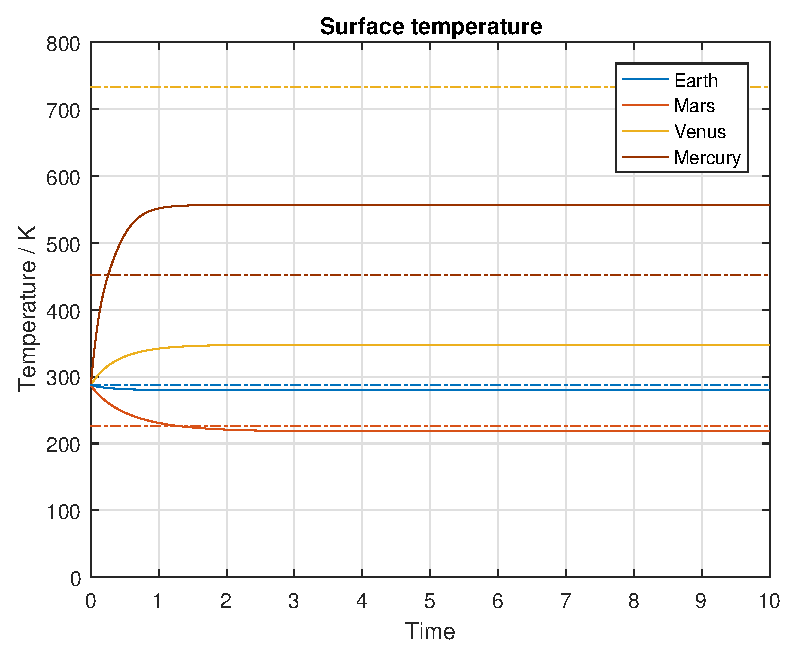
\includegraphics[height=0.45\textheight]{planeten/Matlab/figures/surfaceTemperature.eps}
			\caption{Globale Durchschnittstemperatur}
		\end{figure}
		
		\begin{figure}
			\center
			\includegraphics[height=0.45\textheight]{planeten/Matlab/figures/humidity.eps}
			\caption{Relative Luftfeuchtigkeit}
		\end{figure}
		
		\begin{figure}
			\center
			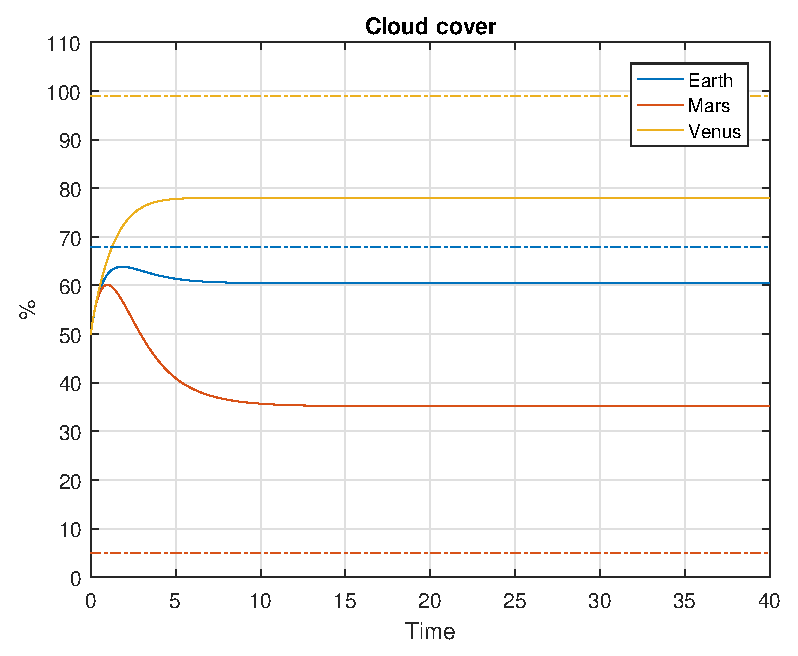
\includegraphics[height=0.45\textheight]{planeten/Matlab/figures/cloudCover.eps}
			\caption{Prozentuale Wolkenabdeckung}
		\end{figure}
		
		\begin{figure}
			\center
			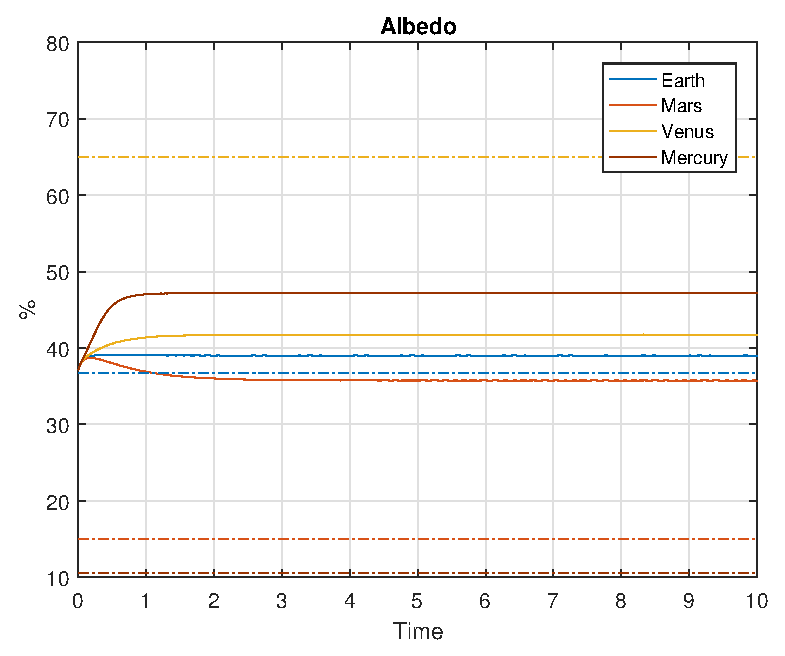
\includegraphics[height=0.45\textheight]{planeten/Matlab/figures/albedo.eps}
			\caption{Albedo}
		\end{figure}

\section{Schlussfolgerung}
\rhead{Schlussfolgerung}

Ergebnisse gleichen dem heutigen Status
Extremes Klima von Mars \& Venus vermutlich prädestiniert

Abweichungen

Ergebnisse nur mit Vorsicht zu geniessen

Nicht modelierte faktoren:
Nur Wasser simuliert
Chemische und Physikalische Vorgänge bei extremen Temperaturen

Andere Treibhausgase wie CO$_2$, welches heute den grössten Anteil der Venus- und Marsatmosphäre ausmacht, vernachlässigt.

\subsection{Verbesserungsmöglichkeiten}

Nächste Schritte das Modell zu verbessern

Um mehr Genauigkeit in den Extremen Bereichen zu erreichen, müssten mehr atmosphärische Gase einbezogen werden.
Diese Gase besitzen wiederum unterschiedliche Gefrierpunkte, was die Modellierung der Vereisung zulässt.
		
Im simulierten Modell wurden lediglich der Durchmesser und die Distanz zur Sonne der Planeten einbezogen. Um die Aussagekraft zu verbessern könnten weitere Planet-abhängige Parameter implementiert werden, wie der Vulkanismus und die Rotationsgeschwindigkeit. Die Rotation erlaubt das Modellieren von Tag- und Nachtseitentemperatur, welche sich stark auf das Klima auswirken.


\printbibliography[heading=subbibliography]
\end{refsection}
